%%%% PLEASE REPLACE ENTIRELY WITH YOUR OWN CONTENT %%%%

\chapter{Introduction}

In recent years, computing has undergone significant evolution, reaching a point where improving the hardware of traditional devices presents considerable challenges. This has driven research in quantum computing, a technology that promises to revolutionize the field by enabling much more efficient calculations and superior processing capabilities. In applications such as molecular simulation, quantum computing has proven to be remarkably more efficient than classical computing, justifying investment in its development.

However, one of the main obstacles of quantum computing is the high cost associated with its devices. To run programs on a quantum computer, it must operate at extremely low temperatures, close to 0.1 Kelvin, which significantly increases the cost and technical complexity. Therefore, methods are being investigated to improve and optimize these devices, making them more accessible and viable for broader use.

Currently, one of the most practical ways to harness quantum computing's potential is through \textbf{quantum simulation}. Quantum simulation allows us to study complex quantum systems using either quantum simulators or classical computers. By emulating the behavior of quantum systems, we can explore quantum algorithms and applications effectively without necessarily requiring a fully functional quantum computer.

The main objective of this project is to develop a quantum simulator capable of efficiently modeling molecules using advanced quantum algorithms, with a specific focus on implementing the Variational Quantum Eigensolver (VQE) algorithm. This algorithm combines quantum circuits for state preparation and classical optimizers that adjust parameters to minimize the system's energy. Additionally, the project introduces innovations in the design of adaptive quantum circuits, the integration of simultaneous optimizations of nuclear and electronic coordinates, all within a modular and extensible project structure that allows for easy and effective adaptation of the simulation.

\section{Work goals}
The primary goal of this project is to contribute a novel methodology to the field of molecular simulations by:

\begin{itemize}
  \item Optimize the quantum simulation framework to minimize computational overhead while maintaining accuracy in modeling molecular systems, focusing on enhancing the Variational Quantum Eigensolver (VQE) efficiency.
  \item Develop an adaptive quantum ansatz capable of dynamically selecting and integrating operators with the highest impact on performance, ensuring rapid convergence and reduced computational cost.
  \item Integrate advanced hybrid optimization cycles that streamline both electronic state and nuclear geometry refinements, with an emphasis on computational speed and scalability.
  \item Design a high-performance, modular architecture tailored for extensibility, facilitating the efficient inclusion of cutting-edge algorithms, ansatz designs, and optimization strategies.
\end{itemize}


\section{Requirements and specifications}

To achieve these objectives, the following requirements and specifications have been established:

\begin{itemize}
  \item \textbf{Dynamic Ansatz Construction}: Integrate an adaptive ansatz mechanism that employs energy gradient calculations to iteratively select and include the most impactful operators, reducing the complexity of the quantum circuits without compromising accuracy.
  \item \textbf{Advanced Hybrid Optimization}: Develop a unified optimization cycle combining variational parameter updates and nuclear geometry refinements, supported by precise gradient-based techniques. Ensure the use of optimizers for rapid convergence and enhanced stability.
  \item \textbf{Scalable Hamiltonian Management}: Implement a modular Hamiltonian construction process that accommodates different molecular geometries and basis sets with efficient computation of molecular properties.
  \item \textbf{Efficient Gradient Computation}: Optimize gradient calculations for both quantum and nuclear coordinates using automatic differentiation, enabling simultaneous updates and faster convergence.
  \item \textbf{Performance Monitoring and Visualization}: Develop tools for tracking energy convergence, execution time, and molecular geometry evolution. Include detailed visualizations (e.g., energy evolution plots, 3D geometries) to ensure transparency and allow performance analysis.
  \item \textbf{Extensibility and Modularity}: Ensure a modular project structure that facilitates the inclusion of new ansatz types, optimizers, and molecular systems with minimal adjustments. Employ a structured directory for clear separation of functionality and scalability.
  \item \textbf{Parallel Execution Capability}: Leverage multiprocessing capabilities to evaluate multiple optimizers and configurations in parallel, enabling comprehensive performance analysis across various configurations.
\end{itemize}


\section{Methods and procedures}

In our project, we have implemented a series of advanced methodologies that integrate quantum and classical techniques with specific innovations to address molecular optimization problems and energy calculations efficiently. We have combined quantum computing, which enables the evaluation of fundamental system properties such as energy and quantum states, with classical algorithms that optimize the parameters required to represent these states effectively. This hybrid approach, inspired by the ideas of Richard Feynman, has been validated in works like that of Arute et al. (2019), who achieved quantum supremacy using digital circuits to solve problems inaccessible to classical computers. Within this framework, we used the Variational Quantum Eigensolver (VQE) algorithm as the core of our simulation. This algorithm combines parameterized circuits, known as ansatz, with classical optimization to minimize the expected value of the molecular Hamiltonian, which describes the total energy of the system. Introduced by Peruzzo et al. in 2014, VQE has proven particularly effective for noisy intermediate-scale quantum (NISQ) devices.

Additionally, we have implemented an adaptive ansatz that enhances efficiency by dynamically constructing the quantum circuit. This ansatz iteratively selects relevant operators based on energy gradients, an approach inspired by the ADAPT-VQE algorithm by Grimsley et al. (2019), ensuring faster and more accurate convergence to the ground state. Since scalable quantum hardware is not available, we used classical simulators such as PennyLane's default.qubit to emulate digital quantum circuits. This has allowed us to design and evaluate algorithms robustly in classical environments while maintaining the ability to test innovative approaches.

Among the main innovations implemented, we developed a dynamic adaptive ansatz that incorporates only the quantum operators with the greatest impact on energy, calculated through gradients using automatic differentiation. This not only optimizes computational efficiency but also reduces the complexity of the model. We also implemented a hybrid optimization cycle that simultaneously adjusts the ansatz parameters and nuclear positions, accurately capturing the interaction between electrons and molecular geometry. The modular structure of the code has been key to enabling the incorporation of new functionalities and the comparison of different optimization strategies without affecting other components of the system. Finally, we designed the system to support multiple types of ansatz and optimizers, facilitating an exhaustive comparative analysis and ensuring the scalability of the project for future extensions in quantum chemistry and molecular simulations.

\section{Work plan}

During the development of the project, the initial plan was largely followed. However, several complications arose that extended some deadlines, requiring adjustments to the overall timeline to achieve the established objectives.

The main setback was related to the integration of the JAX interface. From the outset, we were confident that using JAX would significantly improve the performance of the simulations. However, upon completing the initial integration, we were surprised to find that the performance not only failed to improve but actually worsened. This unexpected result led us to conduct more checks than initially planned, aiming to verify the accuracy of the results and identify the root cause of this behavior.

This situation caused delays in the second phase of the project, which, in turn, required a reduction in the time allocated to the third phase to meet the deadlines. Despite this, we decided not to compromise on the quality of the project. As a result, the overall development time had to be extended, increasing the daily hours dedicated to the project. This additional effort ensured that the initial objectives were achieved without compromising the proposed quality standards.

\begin{figure}[H]
  \centering
  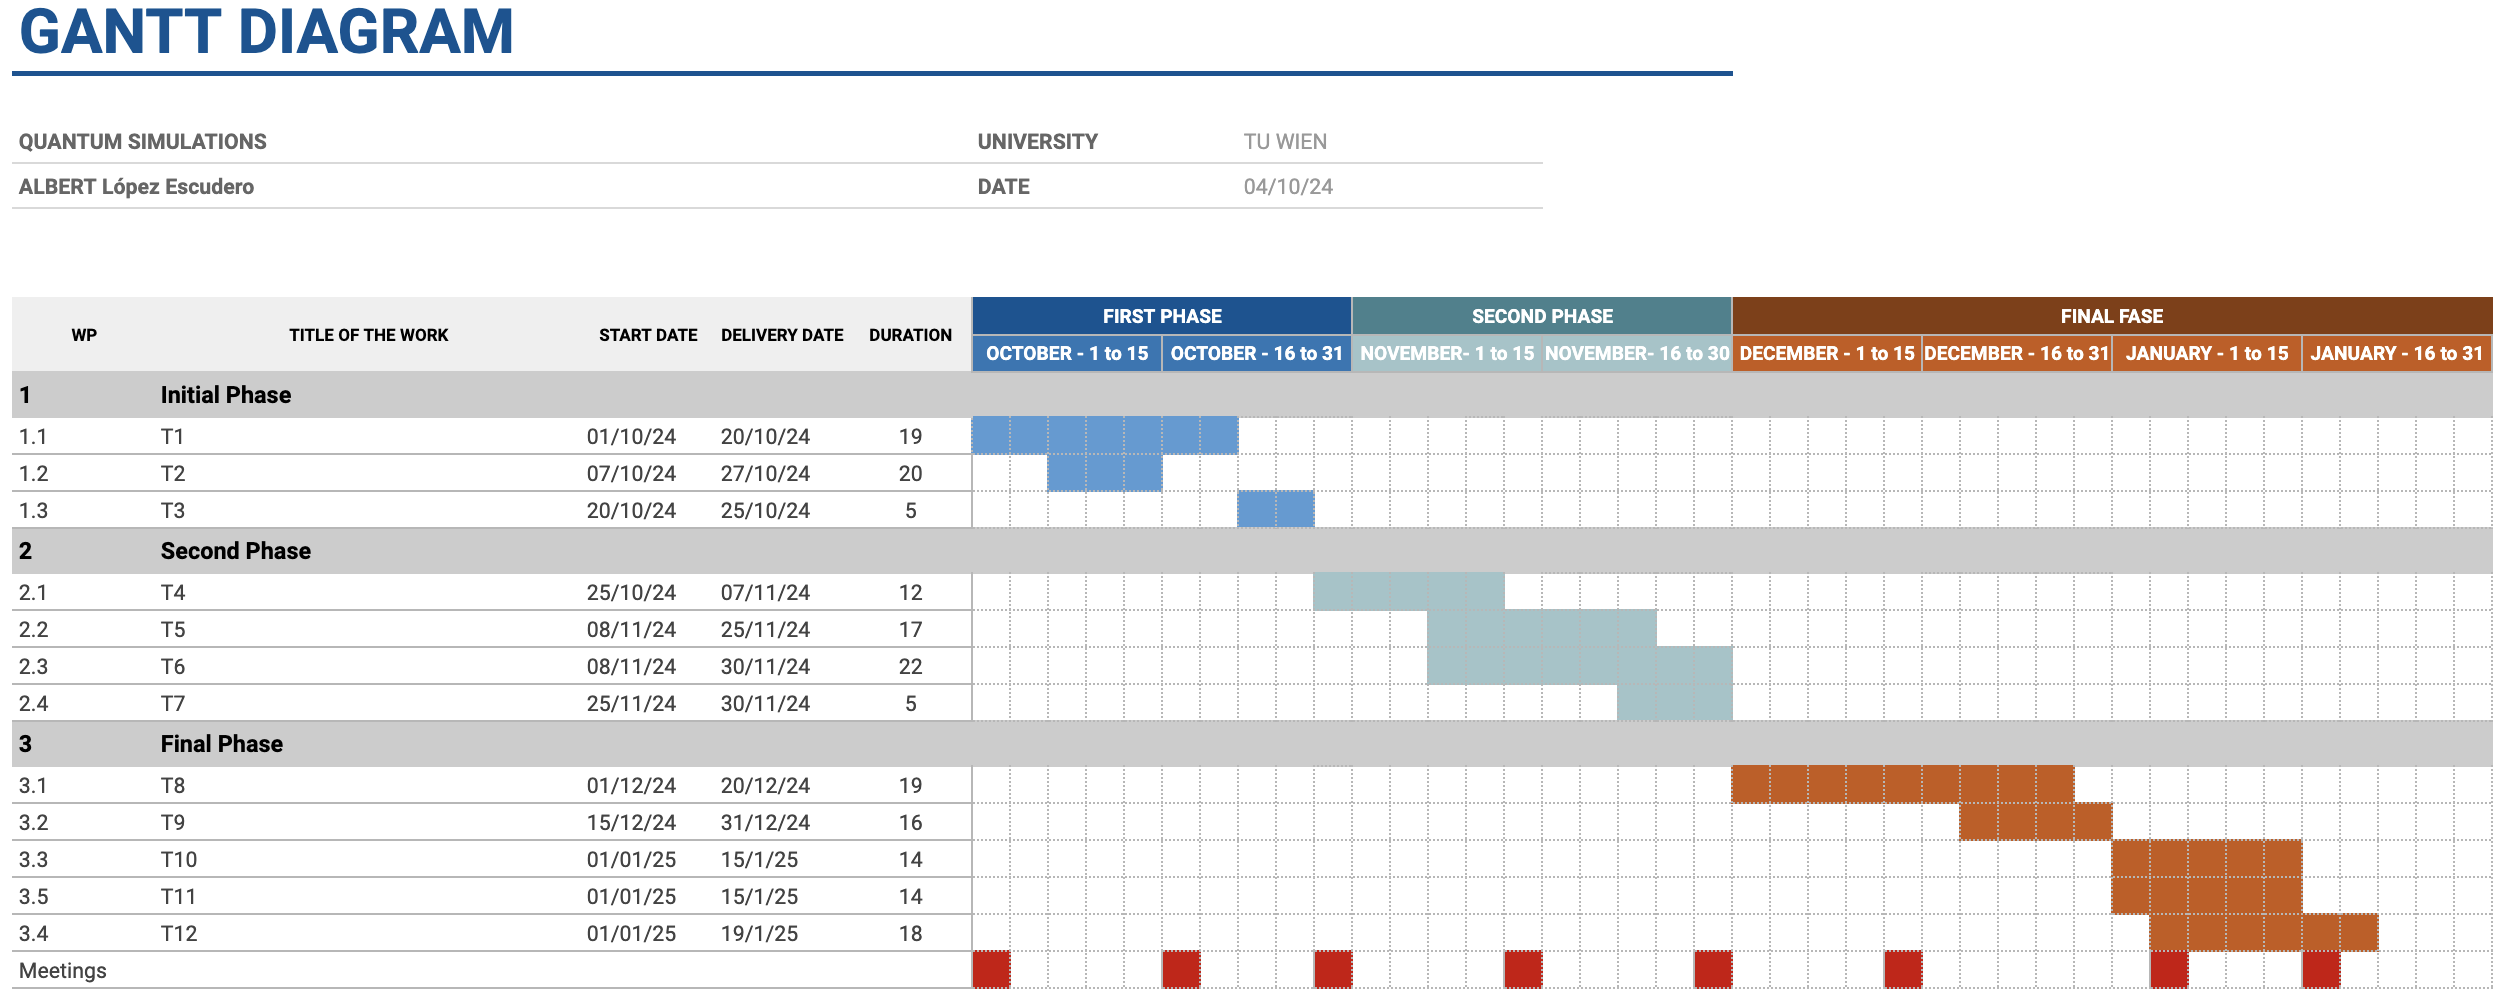
\includegraphics[width=1\textwidth]{img/Gantt_diagram.png}
  \caption{Gantt diagram showing the project timeline and the distribution of tasks over the development period.}
  \label{fig:gantt_diagram}
\end{figure}